\documentclass{standalone}
\usepackage{tikz}
\usetikzlibrary{patterns, positioning}


\begin{document}
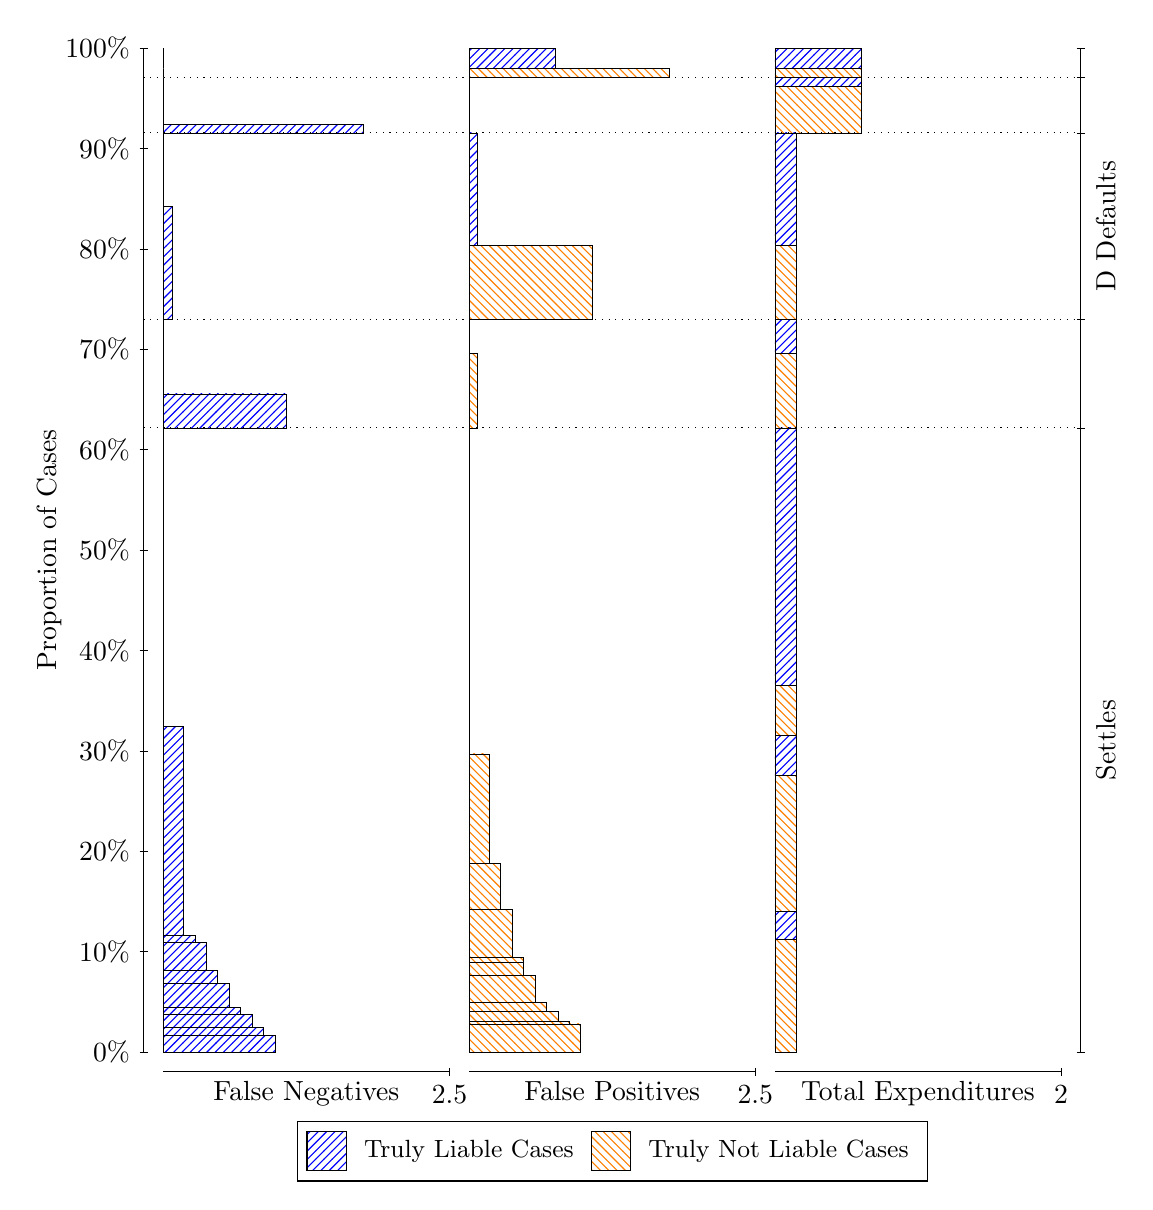
\begin{tikzpicture}
\draw[black, very thin] (1.5,1.75) -- (1.5,14.5);
\node[rotate=90, text=black, anchor=center] at (0.3, 8.125) {Proportion of Cases};
\draw[black, very thin] (1.45,1.75) -- (1.55,1.75);
\node[text=black, anchor=east] at (1.45, 1.75) {0\%};
\draw[black, very thin] (1.45,3.025) -- (1.55,3.025);
\node[text=black, anchor=east] at (1.45, 3.025) {10\%};
\draw[black, very thin] (1.45,4.3) -- (1.55,4.3);
\node[text=black, anchor=east] at (1.45, 4.3) {20\%};
\draw[black, very thin] (1.45,5.575) -- (1.55,5.575);
\node[text=black, anchor=east] at (1.45, 5.575) {30\%};
\draw[black, very thin] (1.45,6.85) -- (1.55,6.85);
\node[text=black, anchor=east] at (1.45, 6.85) {40\%};
\draw[black, very thin] (1.45,8.125) -- (1.55,8.125);
\node[text=black, anchor=east] at (1.45, 8.125) {50\%};
\draw[black, very thin] (1.45,9.4) -- (1.55,9.4);
\node[text=black, anchor=east] at (1.45, 9.4) {60\%};
\draw[black, very thin] (1.45,10.675) -- (1.55,10.675);
\node[text=black, anchor=east] at (1.45, 10.675) {70\%};
\draw[black, very thin] (1.45,11.95) -- (1.55,11.95);
\node[text=black, anchor=east] at (1.45, 11.95) {80\%};
\draw[black, very thin] (1.45,13.225) -- (1.55,13.225);
\node[text=black, anchor=east] at (1.45, 13.225) {90\%};
\draw[black, very thin] (1.45,14.5) -- (1.55,14.5);
\node[text=black, anchor=east] at (1.45, 14.5) {100\%};

\draw[black, very thin] (13.4,1.75) -- (13.4,14.5);
\draw[black, very thin] (13.35,1.75) -- (13.45,1.75);
\node[anchor=west] at (13.35, 1.75) {};
\draw[black, very thin] (13.35,9.6756) -- (13.45,9.6756);
\node[anchor=west] at (13.35, 9.6756) {};
\draw[black, very thin] (13.35,11.055) -- (13.45,11.055);
\node[anchor=west] at (13.35, 11.055) {};
\draw[black, very thin] (13.35,13.423) -- (13.45,13.423);
\node[anchor=west] at (13.35, 13.423) {};
\draw[black, very thin] (13.35,14.127) -- (13.45,14.127);
\node[anchor=west] at (13.35, 14.127) {};
\draw[black, very thin] (13.35,14.5) -- (13.45,14.5);
\node[anchor=west] at (13.35, 14.5) {};

\draw[black, very thin, pattern color=blue, pattern=north east lines] (1.75,1.75) rectangle (3.167,1.9581);
\draw[black, very thin, pattern color=blue, pattern=north east lines] (1.75,1.9581) rectangle (3.0217,2.0622);
\draw[black, very thin, pattern color=blue, pattern=north east lines] (1.75,2.0622) rectangle (2.8763,2.2292);
\draw[black, very thin, pattern color=blue, pattern=north east lines] (1.75,2.2292) rectangle (2.731,2.3163);
\draw[black, very thin, pattern color=blue, pattern=north east lines] (1.75,2.3163) rectangle (2.5857,2.6199);
\draw[black, very thin, pattern color=blue, pattern=north east lines] (1.75,2.6199) rectangle (2.4403,2.7835);
\draw[black, very thin, pattern color=blue, pattern=north east lines] (1.75,2.7835) rectangle (2.295,3.1448);
\draw[black, very thin, pattern color=blue, pattern=north east lines] (1.75,3.1448) rectangle (2.1497,3.2316);
\draw[black, very thin, pattern color=blue, pattern=north east lines] (1.75,3.2316) rectangle (2.0043,5.8896);
\draw[black, very thin, pattern color=orange, pattern=north west lines] (1.75,5.8896) rectangle (1.75,9.6756);
\draw[black, very thin, pattern color=blue, pattern=north east lines] (1.75,9.6756) rectangle (3.3123,10.107);
\draw[black, very thin, pattern color=orange, pattern=north west lines] (1.75,10.107) rectangle (1.75,11.055);
\draw[black, very thin, pattern color=blue, pattern=north east lines] (1.75,11.055) rectangle (1.859,12.484);
\draw[black, very thin, pattern color=orange, pattern=north west lines] (1.75,12.484) rectangle (1.75,13.423);
\draw[black, very thin, pattern color=blue, pattern=north east lines] (1.75,13.423) rectangle (4.2933,13.535);
\draw[black, very thin, pattern color=orange, pattern=north west lines] (1.75,13.535) rectangle (1.75,14.127);
\draw[black, very thin, pattern color=orange, pattern=north west lines] (1.75,14.127) rectangle (1.75,14.238);
\draw[black, very thin, pattern color=blue, pattern=north east lines] (1.75,14.238) rectangle (1.75,14.5);
\draw[black, very thin, pattern color=orange, pattern=north west lines] (5.6333,1.75) rectangle (7.0503,2.1067);
\draw[black, very thin, pattern color=orange, pattern=north west lines] (5.6333,2.1067) rectangle (6.905,2.1375);
\draw[black, very thin, pattern color=orange, pattern=north west lines] (5.6333,2.1375) rectangle (6.7597,2.2673);
\draw[black, very thin, pattern color=orange, pattern=north west lines] (5.6333,2.2673) rectangle (6.6143,2.3814);
\draw[black, very thin, pattern color=orange, pattern=north west lines] (5.6333,2.3814) rectangle (6.469,2.7203);
\draw[black, very thin, pattern color=orange, pattern=north west lines] (5.6333,2.7203) rectangle (6.3237,2.8862);
\draw[black, very thin, pattern color=orange, pattern=north west lines] (5.6333,2.8862) rectangle (6.3237,2.9487);
\draw[black, very thin, pattern color=orange, pattern=north west lines] (5.6333,2.9487) rectangle (6.1783,3.5567);
\draw[black, very thin, pattern color=orange, pattern=north west lines] (5.6333,3.5567) rectangle (6.033,4.1464);
\draw[black, very thin, pattern color=orange, pattern=north west lines] (5.6333,4.1464) rectangle (5.8877,5.536);
\draw[black, very thin, pattern color=blue, pattern=north east lines] (5.6333,5.536) rectangle (5.6333,9.6756);
\draw[black, very thin, pattern color=orange, pattern=north west lines] (5.6333,9.6756) rectangle (5.7423,10.623);
\draw[black, very thin, pattern color=blue, pattern=north east lines] (5.6333,10.623) rectangle (5.6333,11.055);
\draw[black, very thin, pattern color=orange, pattern=north west lines] (5.6333,11.055) rectangle (7.1957,11.994);
\draw[black, very thin, pattern color=blue, pattern=north east lines] (5.6333,11.994) rectangle (5.7423,13.423);
\draw[black, very thin, pattern color=orange, pattern=north west lines] (5.6333,13.423) rectangle (5.6333,14.015);
\draw[black, very thin, pattern color=blue, pattern=north east lines] (5.6333,14.015) rectangle (5.6333,14.127);
\draw[black, very thin, pattern color=orange, pattern=north west lines] (5.6333,14.127) rectangle (8.1767,14.238);
\draw[black, very thin, pattern color=blue, pattern=north east lines] (5.6333,14.238) rectangle (6.7233,14.5);
\draw[black, very thin, pattern color=orange, pattern=north west lines] (9.5167,1.75) rectangle (9.7892,3.1761);
\draw[black, very thin, pattern color=blue, pattern=north east lines] (9.5167,3.1761) rectangle (9.7892,3.5344);
\draw[black, very thin, pattern color=orange, pattern=north west lines] (9.5167,3.5344) rectangle (9.7892,5.2628);
\draw[black, very thin, pattern color=blue, pattern=north east lines] (9.5167,5.2628) rectangle (9.7892,5.7745);
\draw[black, very thin, pattern color=orange, pattern=north west lines] (9.5167,5.7745) rectangle (9.7892,6.4059);
\draw[black, very thin, pattern color=blue, pattern=north east lines] (9.5167,6.4059) rectangle (9.7892,9.6756);
\draw[black, very thin, pattern color=orange, pattern=north west lines] (9.5167,9.6756) rectangle (9.7892,10.623);
\draw[black, very thin, pattern color=blue, pattern=north east lines] (9.5167,10.623) rectangle (9.7892,11.055);
\draw[black, very thin, pattern color=orange, pattern=north west lines] (9.5167,11.055) rectangle (9.7892,11.994);
\draw[black, very thin, pattern color=blue, pattern=north east lines] (9.5167,11.994) rectangle (9.7892,13.423);
\draw[black, very thin, pattern color=orange, pattern=north west lines] (9.5167,13.423) rectangle (10.607,14.015);
\draw[black, very thin, pattern color=blue, pattern=north east lines] (9.5167,14.015) rectangle (10.607,14.127);
\draw[black, very thin, pattern color=orange, pattern=north west lines] (9.5167,14.127) rectangle (10.607,14.238);
\draw[black, very thin, pattern color=blue, pattern=north east lines] (9.5167,14.238) rectangle (10.607,14.5);
\draw[black, dotted] (1.5,9.6756) -- (13.4,9.6756);
\draw[black, dotted] (1.5,11.055) -- (13.4,11.055);
\draw[black, dotted] (1.5,13.423) -- (13.4,13.423);
\draw[black, dotted] (1.5,14.127) -- (13.4,14.127);
\draw[black, very thin] (1.75,1.5) -- (5.3833,1.5);
\node[text=black, anchor=north] at (3.5667, 1.5) {False Negatives};
\draw[black, very thin] (5.3833,1.45) -- (5.3833,1.55);
\node[text=black, anchor=north] at (5.3833, 1.45) {2.5};

\draw[black, very thin] (5.6333,1.5) -- (9.2667,1.5);
\node[text=black, anchor=north] at (7.45, 1.5) {False Positives};
\draw[black, very thin] (9.2667,1.45) -- (9.2667,1.55);
\node[text=black, anchor=north] at (9.2667, 1.45) {2.5};

\draw[black, very thin] (9.5167,1.5) -- (13.15,1.5);
\node[text=black, anchor=north] at (11.333, 1.5) {Total Expenditures};
\draw[black, very thin] (13.15,1.45) -- (13.15,1.55);
\node[text=black, anchor=north] at (13.15, 1.45) {2};

\node[text=black, centered, rotate=90] at (13.72, 5.7128) {Settles};

\node[text=black, centered, rotate=90] at (13.72, 12.239) {D Defaults};



\draw (7.449999999999999,1.5) node[draw=none] (baseCoordinate) {};
\begin{scope}[align=center]
        \matrix[scale=0.5, draw=black, below=0.5cm of baseCoordinate, nodes={draw}, column sep=0.1cm]{
            \node[rectangle, draw, minimum width=0.5cm, minimum height=0.5cm, pattern color=blue, pattern=north east lines] {}; &
            \node[draw=none, font=\small, text=black] (B) {Truly Liable Cases}; &
            \node[rectangle, draw, minimum width=0.5cm, minimum height=0.5cm, pattern color=orange, pattern=north west lines] {}; &
            \node[draw=none, font=\small, text=black] (B) {Truly Not Liable Cases}; \\
            };
\end{scope}

\end{tikzpicture}
\end{document}